\chapter{精密直线运动平台动力学建模与参数辨识}
\section{引言}
为了实现精密直线运动平台的高性能控制,了解与掌握被控对象的系统特性显得尤为重要,准确地建模与参数辨识成为实际工业应用环境中发挥先进控制方法优势的有力保障。
精密直线运动平台的典型代表就是永磁同步直线电机(Permanent Magnet Synchronous Linear Motors, PMLSMs),本文也以PMLSMs为例,后文提到的精密直线运动平台均指PMLSMs。

本章首先分析了精密直线运动平台基本工作原理。然后根据牛顿第二定律对精密直线运动平台进行了动力学建模,同时,分析了其典型的扰动类型,主要包括定位力\cite{zhao2005adaptive,chen2009modeling,bascetta2009force,hu2009coordinated,yao2011adaptive}、摩擦力\cite{de1995new}、模型参数摄动以及电磁非线性引起的扰动\cite{kano2005simple}。为了更方便地描述各种扰动与不确定性的影响,将其归纳为内部和外部的集总扰动。根据扰动与时间的关系,进一步将集总扰动分为时变的和时不变的两部分。最后,总结了辨识常用的几种方法,并对实验对象进行了初步的系统辨识实验,获得了系统等效质量、等效阻尼以及定位力的空间周期系统模型信息。为后续控制方法的研究奠定了基础。
\section{精密直线运动平台工作原理}
\begin{comment}
\subsection{架构组成}
精密直线运动平台系统架构主要包括机械结构、电气结构和软件控制架构,如图\ref{C2_01}所示。各部分具体描述如下:
\begin{figure}[H]
	\centering
	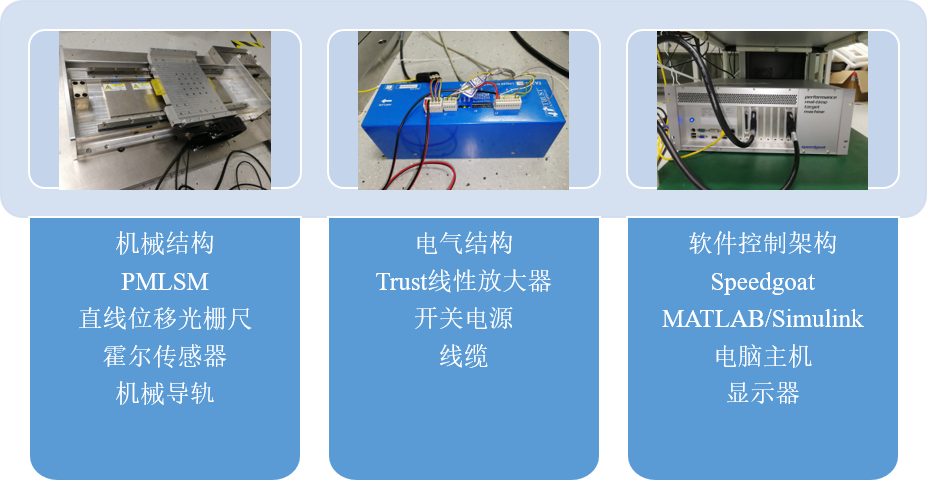
\includegraphics[width=12cm]{figures/平台架构}
	\caption{精密直线运动平台系统架构.}
	\label{C2_01}
\end{figure}

本文所述精密直线运动平台的机械结构主要是指PMLSMs,具体是指Akribis公司研发的ACM1-L100-TL80有铁芯PMLSMs,包括定子和动子,动子是由电枢线圈三相绕组、霍尔传感器以及光栅尺读数头组成;定子是由钕铁硼(NdFeB)永磁序列、导轨和直线位移光栅尺组成。ACM1-L100-TL80的具体规格参数如表\ref{T2-01}所示。
\begin{table}[H]
	\caption{ACM1-L100-TL80规格参数.}
	\label{T2-01}
	\centering
	\setlength{\tabcolsep}{5mm}
	\begin{tabular}{ccc}
		\toprule[1.5pt]
		规格参数 &值  &单位 \\
		\midrule
		%\hline
%		电机常数&33.1&$\text{N/SqRt(W)}$\\
		力常数&72.9&$\text{N/Arms}$\\
		极距&20.0&$\text{mm}$\\
		电感&18.2&$\text{mH}$\\
		最大总线电压&600&$\text{Vdc}$\\
		持续力&306.3&$\text{N}$\\
		峰值力&1321.8&$\text{N}$\\
%		持续功率&85.6&$\text{W}$\\
%		峰值功率&1593.3&$\text{W}$\\
		持续电流&4.2&$\text{Arms}$\\
        峰值电流&19.2&$\text{Arms}$\\
		反电动势常数&59.5&$\text{Vpeak/m/s}$\\
	    电气时间常数&3.8&$\text{ms}$\\
%热耗散常数&1.1&$\text{W/\SI{}{\degreeCelsius}}$\\
%磁吸引力&3091.0&$\text{N}$\\
		\bottomrule[1.5pt]
	\end{tabular}
\end{table}
本文所述精密直线运动平台的电气结构主要包括开关电源和Trust线性放大器,具体是指Trust公司TA310型号的线性伺服放大器,其内部嵌入了自动对相算法,能够保证电气系统上电之后,PMLSM即可实现自动对相,即可以自动搜索到保证所处位置最大出力的电流初始相位角,从而保证Trust线性放大器的有效功率最大。TA310的规格参数如表\ref{T2-02}所示。
\begin{table}[H]
	\caption{TA310规格参数.}
	\label{T2-02}
	\centering
	\setlength{\tabcolsep}{5mm}
	\begin{tabular}{ccc}
		\toprule[1.5pt]
		规格参数 &值  &单位 \\
		\midrule
		%\hline
		电源电压&15-48&$\text{V}$\\
		等效电机电压&$\le43$&$\text{V}$\\
		峰值电流&$\pm$8&$\text{A}$\\
		输入电压&$\pm10$&$\text{V}$\\
		电压-电流转换系数&$0.2-0.8$&$\text{V}$\\
		带宽&5&$\text{kHz}$\\
		\bottomrule[1.5pt]
	\end{tabular}
\end{table}

本文所述精密直线运动平台的软件控制架构主要包括电脑主机、Speedgoat实时控制系统、MATLAB/Simulink以及显示器。其中Speedgoat实时控制系统是由瑞士公司Speedgoat开发的一套实时控制系统开发与快速验证的设备,能够与MATLAB/Simulink无缝连接,极大地方便了先进控制方法的验证与实现,因此,本文所有提出的控制方法都是基于这一完整的实时控制系统进行实验验证与实现。

为了更直观地表示所述精密直线运动平台系统整体控制架构,如图\ref{精密直线运动平台系统信号流图}所示,本文在此给出所述精密直线运动平台系统各部分之间的信号流图,即系统架构各组成部分之间的连接关系和信号交互模式。
\begin{figure}[H]
	\centering
	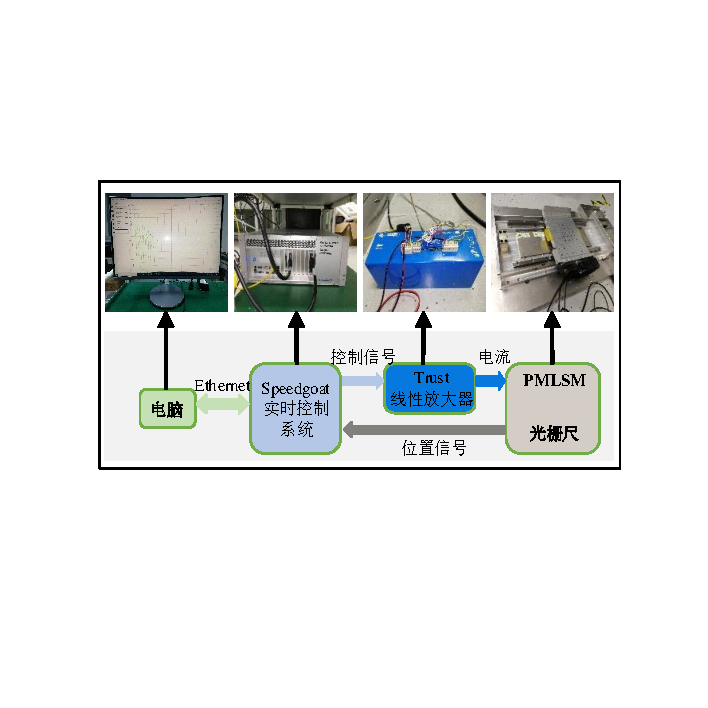
\includegraphics[width=12cm]{figures/实验装置图.pdf}
	\caption{精密直线运动平台系统信号流图.}
	\label{精密直线运动平台系统信号流图}
\end{figure}
\end{comment}

%\subsection{工作原理}
精密直线运动平台的工作原理与旋转永磁同步电机类似,均来自矢量变换控制原理。矢量变换控制的基本思想为:
通过建立合适的坐标系($dq$轴),利用坐标变换工具,将交流三相绕组中的电流转换为两相直流绕组中的电流,这样既能够达到降维的目的,又能够减少耦合,能够极大地简化精密直线运动平台的模型。
\begin{comment}
通过数学上的坐标变换方法,可以实现交流三相到直流两相的转化,实现降维和解耦的目的,大大简化系统模型。
\end{comment}
精密直线运动平台的矢量控制中,将其三相电流合成出力电流矢量,定位于磁场的$q$轴,而令$d$轴励磁电流矢量为$0$,这样,PMLSMs就可以按照直流电机的方式进行控制,其出力为水平向力。PMLSMs通常采用$i_d=0$控制模式,也是最大力控制。这里值得注意的是,如果$i_d\neq0$,会使得永磁产生退磁现象。

如图\ref{dq轴示意图}所示,为永磁序列的磁通密度空间分布示意图,电机水平沿X向运动,水平磁通密度$B_x$和垂向磁通密度$B_z$都近似为正弦分布,且$B_z$空间相角超前于$B_x$空间相角90度。图中对PMLSMs进行矢量控制时永磁阵列表面空间的$d$、$q$轴定义进行了说明,其中磁通密度在垂向和水平向的正方向分别定义为沿Z轴正向和沿X轴正向。

	$\bullet$ 精密直线运动平台的$d$轴定义为:永磁阵列表面空间磁场中垂向磁通密度$B_z$正向最大位置,此时磁通密度$B_x$为0;
	
	$\bullet$ 精密直线运动平台的$q$轴定义为:$B_z$为0的位置,此时磁通密度$B_x$为正向最大。

% TODO: \usepackage{graphicx} required
\begin{figure}[H]
	\centering
	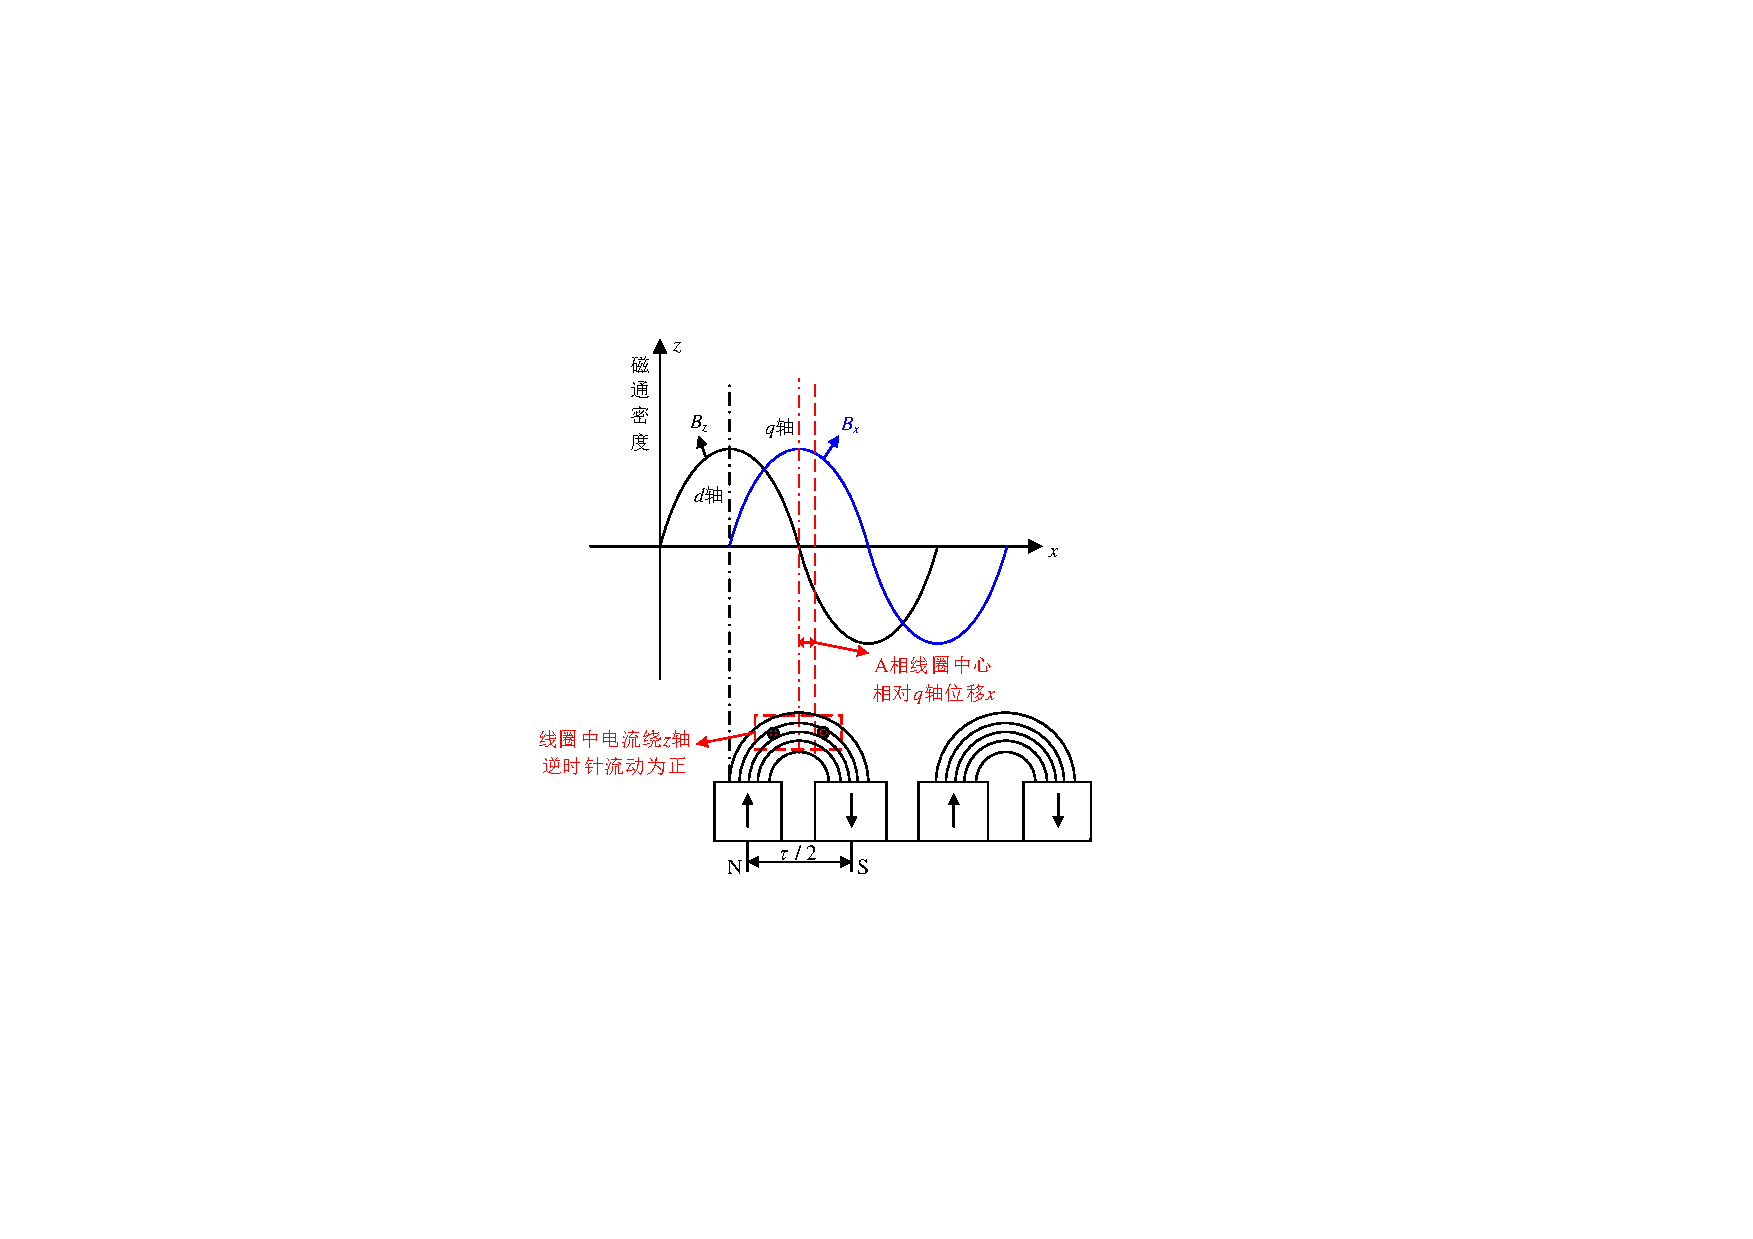
\includegraphics[width=12cm]{figures/dq轴示意图.pdf}
	\caption{dq轴示意图.}
	\label{dq轴示意图}
\end{figure}




电机三相中的变量和$d$、$q$轴中的变量关系如图\ref{三相变量与dq轴变量}所示。
\begin{figure}[H]
	\centering
	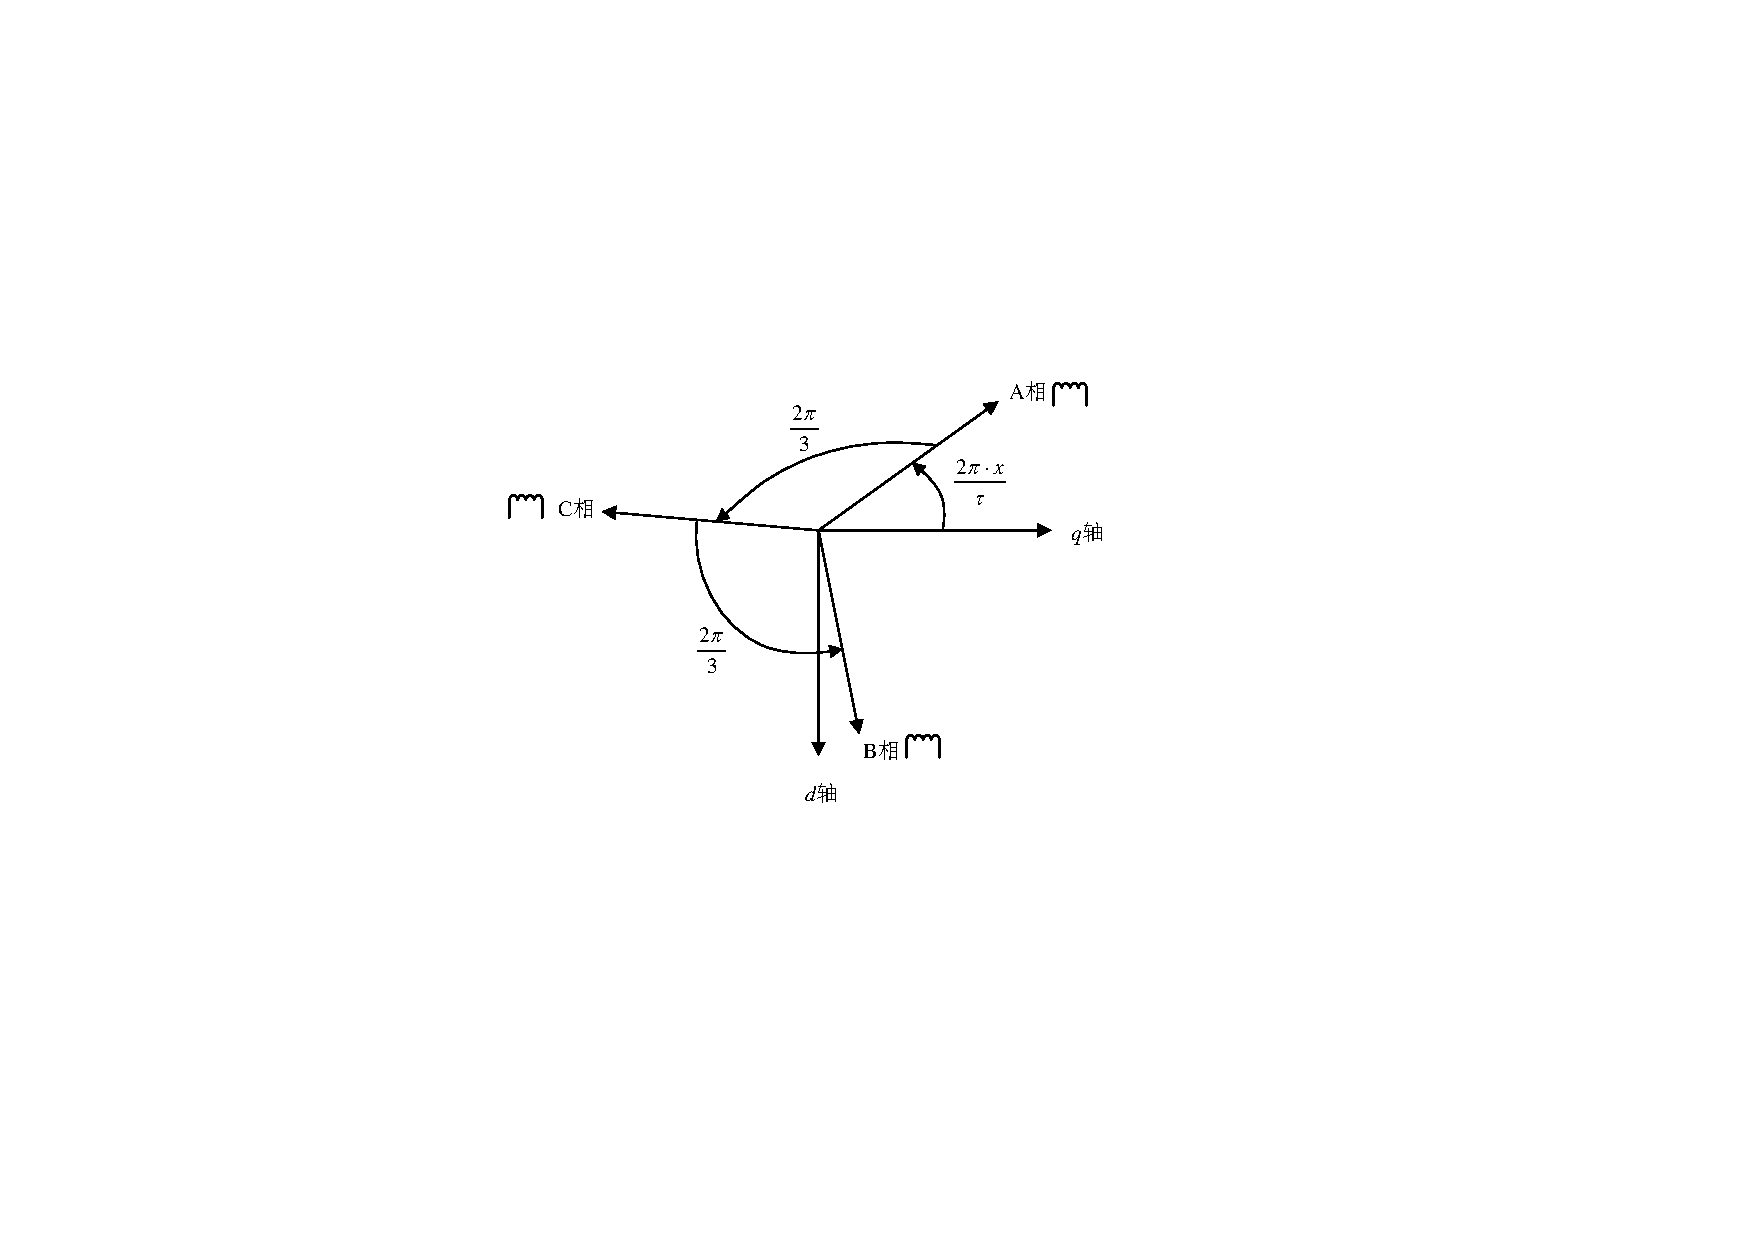
\includegraphics[width=12cm]{figures/三相变量与dq轴变量.pdf}
	\caption{三相变量与$dq$轴变量.}
	\label{三相变量与dq轴变量}
\end{figure}

在直线运动平台的矢量控制中,旋转磁动势作为等效衡量准则,通过Clark变换\cite{阮毅2016电力拖动自动控制系统},可以将三相交流电流$i_a$、$i_b$、$i_c$转化成两相交流电流$i_\alpha$、$i_\beta$,再通过坐标变换,可以等效成正交坐标系上的直流电流$i_d$和$i_q$。由于直流电流$i_d$和$i_q$相互正交,这样交流电机和直流电机就有类似之处。既然如此,从控制的角度讲,就可以实现以“直流控交流”的目的,因为交流-直流-交流这一变换的对象为电流矢量,所以这种通过坐标变换实现的交直流转化控制系统称为矢量控制系统。


将三相变量和$d$、$q$轴变量中的Clark变换统一到一起,称为Park变换\cite{阮毅2016电力拖动自动控制系统},以三相电流为例,其Park变换为
\begin{equation}
\begin{bmatrix}
i_{d} \\
i_{q} \\
i_{0}
\end{bmatrix}=\frac{2}{3}\cdot
\begin{bmatrix}
\cos \left(\frac{\pi x}{\tau}\right) & \cos \left(\frac{\pi x}{\tau}+\frac{2}{3} \pi\right) & \cos \left(\frac{\pi x}{\tau}+\frac{2}{3} \pi\right) \\
-\sin \left(\frac{\pi x}{\tau}\right) & -\sin \left(\frac{\pi x}{\tau}+\frac{2}{3} \pi\right) & -\sin \left(\frac{\pi x}{\tau}+\frac{2}{3} \pi\right) \\
0.5 & 0.5 & 0.5
\end{bmatrix}
\begin{bmatrix}
i_{a} \\
i_{b} \\
i_{c}
\end{bmatrix}
\end{equation}

Park变换的逆变换为
\begin{equation}
\begin{bmatrix}
	i_{a} \\
	i_{b} \\
	i_{c}
\end{bmatrix}=
\begin{bmatrix}
	\cos \left(\frac{\pi x}{\tau}\right) & -\sin \left(\frac{\pi x}{\tau}\right) & 1 \\
	\cos \left(\frac{\pi x}{\tau}+\frac{2}{3} \pi\right) & -\sin \left(\frac{\pi x}{\tau}+\frac{2}{3} \pi\right) & 1 \\
	\cos \left(\frac{\pi x}{\tau}-\frac{2}{3} \pi\right) & -\sin \left(\frac{\pi x}{\tau}-\frac{2}{3} \pi\right) & 1
\end{bmatrix}
\begin{bmatrix}
	i_{d} \\
	i_{q} \\
	i_{0}
\end{bmatrix}
\end{equation}

一般来说,精密直线运动平台三相绕组为星型连接,满足$i_a+i_b+i_c=0$,则有$i_c=-i_a-i_b$。代入上式进而可简化,因此Park变换可简化为:
\begin{equation}
\begin{bmatrix}
i_{d}\\
i_{q}
\end{bmatrix}=\frac{2}{3}\cdot
\begin{bmatrix}
\cos \left(\frac{\pi x}{\tau}\right)-\cos \left(\frac{\pi x}{\tau}-\frac{2}{3}\pi\right) & \cos \left(\frac{\pi x}{\tau}+\frac{2}{3}\pi\right)-\cos \left(\frac{\pi x}{\tau}-\frac{2}{3}\pi\right) \\
-\sin \left(\frac{\pi x}{\tau}\right)+\sin \left(\frac{\pi x}{\tau}-\frac{2}{3}\pi\right) & -\sin \left(\frac{\pi x}{\tau}+\frac{2}{3}\pi\right)+\sin \left(\frac{\pi x}{\tau}-\frac{2}{3}\pi\right)
\end{bmatrix}
\begin{bmatrix}
i_{a} \\
i_{b}
\end{bmatrix}
\end{equation}
通过三角函数变换,可进一步简化为
\begin{equation}
\begin{bmatrix}
i_{d} \\
i_{q}
\end{bmatrix}=-\frac{2}{\sqrt{3}} \cdot
\begin{bmatrix}
\sin \left(\frac{\pi x}{\tau}-\frac{1}{3}\pi\right) & \sin \left(\frac{\pi x}{\tau}\right) \\
\cos \left(\frac{\pi x}{\tau}-\frac{1}{3} \pi\right) & \cos \left(\frac{\pi x}{\tau}\right)
\end{bmatrix}
\begin{bmatrix}
i_{a} \\
i_{b}
\end{bmatrix}
\end{equation}

由公式(2.1)$\sim$(2.4)可知,在得到交、直流电流设定值$i_q$、$i_d$之后,可通过上述矩阵,得到电机三相电流$i_a$、$i_b$和$i_c$。普通直线电机由于仅在一个方向出力,因此通常直轴电流$i_d$设为0,通过控制算法使得交轴电流$i_q$设为给定电流,进而得到预期的电机出力。

为了更清晰地表达PMLSMs的工作原理,图\ref{PMLSM工作原理}给出了简化后的PMLSM工作原理示意图。
\begin{figure}[!t]
	\centering
	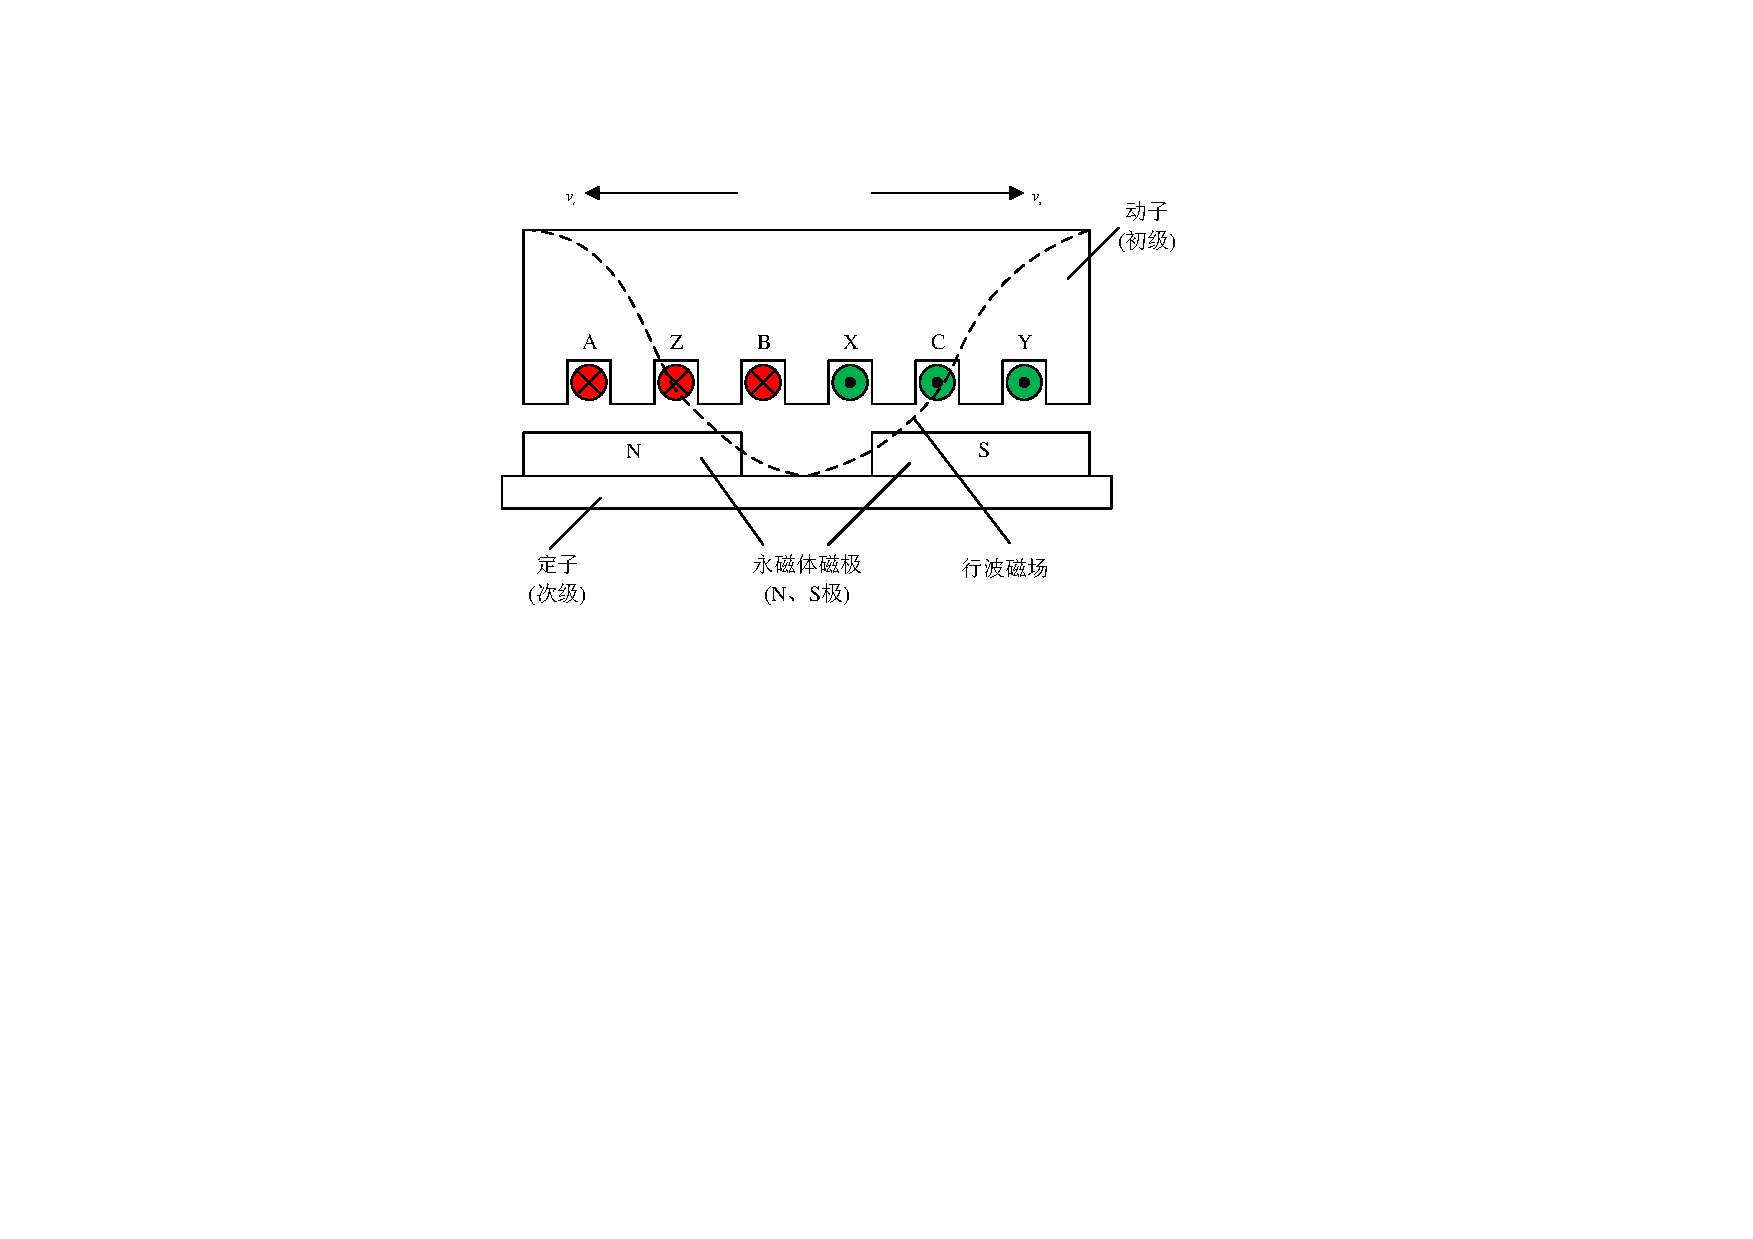
\includegraphics[width=12cm]{figures/PMLSM工作原理示意图.pdf}
	\caption{PMLSM工作原理示意图.}
	\label{PMLSM工作原理}
\end{figure}

在图\ref{PMLSM工作原理}中,A、B、C为三相交流电的相序,在不考虑端部效应的情况下,假设通入绕组的三相交流电为
\begin{equation}
\left\{\begin{aligned}
&i_a=I_m\text{sin}(\frac{2\pi p}{\tau}+\theta_0)\\ 
&i_b=I_m\text{sin}(\frac{2\pi p}{\tau}+\theta_0-2\pi/3)\\ 
&i_c=I_m\text{sin}(\frac{2\pi p}{\tau}+\theta_0-4\pi/3)\\
\end{aligned}\right.
\end{equation}
式中,

$I_m$为电流幅值,单位为(A);

$\tau$为PMLSM极距($\text{m}$);

$p$为PMLSM动子相对于参考原点的相对位置($\text{m}$);

$\theta_0$为$A$相电流初始相位角(rad)。

假设气隙磁密的变化呈标准正弦规律,即,
\begin{equation}
\left\{\begin{aligned}
&B_a=B_m\text{sin}(\frac{2\pi p}{\tau})\\ 
&B_b=B_m\text{sin}(\frac{2\pi p}{\tau}-2\pi/3)\\ 
&B_c=B_m\text{sin}(\frac{2\pi p}{\tau}-4\pi/3)\\
\end{aligned}\right.
\end{equation}
式中,

$B_m$为气隙磁密峰值($\text{T}$);

%$\tau$为PMLSM极距($\text{m}$);
%
%$p$为PMLSM动子相对于参考原点的相对位置($\text{m}$)。

根据洛伦兹原理,三相绕组在正弦磁场中产生的力分别为
\begin{equation}
\left\{\begin{aligned}
&F_a=i_aB_al_{eq}\\ 
&F_b=i_bB_bl_{eq}\\ 
&F_c=i_cB_cl_{eq}\\
\end{aligned}\right.
\end{equation}
式中,$l_{eq}$表示三相绕组在磁场中的等效长度。
  因为每一相产生的力的方向一致,则总的合力为$F=F_a+F_b+F_c$,结合公式(2.5)$\sim$(2.7),可以得出
\begin{equation}
F=\frac{3}{2}I_mB_mL\cos(\theta_0)
\end{equation}

由公式(2.8)可以看出,当$A$相电流的初始相位角能够使得$\cos(\theta_0)=1$时,可以得到最大出力$F_m=\frac{3}{2}I_mB_mL$,这一过程称为电机寻相。在本精密直线平台系统架构中由Trust线性放大器自动完成。

为了统一,后文提到的电磁推力均假设寻相过程已完成,另一方面,由于动圈式PMLSMs系统中,磁场由永磁体产生,因此控制变量仅为通入三相绕组的电流,这样电磁推力可以仅表示为电流的函数,得到电磁推力的简化方程为
\begin{equation}
F_e=K_eI_m
\end{equation}
式中,$K_e$为推力常数,在理想情况下为一正常数;$I_m$为驱动器输出的电流大小。

从上述描述中可以看到,在理想情况下,只需要控制驱动器的电流就可以实现对电机出力的控制,从而实现对PMLSMs的控制,使其在各种输入轨迹的情况下能够实现高性能的跟踪。为了更加了解和掌握被控对象的系统特性,我们仍然需要对其进行动力学建模,并分析其扰动类型,以便更好地对其进行补偿。
\section{精密直线运动平台动力学建模}
%\subsection{动力学建模}
由牛顿第二定律可以得到,精密直线运动平台的动力学方程可表示为
\begin{equation}
M_e\ddot{p}={{F}_{e}}-{{F}_{d}}-{{F}_{f}} 
\end{equation}
式中,

$M_e$为动子的等效质量;

$\ddot{p}$为电机动子的位移;

$F_e$为三相绕组在磁场中产生的电磁推力;

$F_d$为外部扰动,包括线缆力、定位力以及未建模动态等;

$F_f$为非线性摩擦力部分,根据LuGre模型\cite{de1995new},可表示为
\begin{equation}
\label{2.11}
{{F}_{f}}={{F}_{c}}\text{sgn}(v)+({{F}_{s}}-{{F}_{c}}){{e}^{-{{(v/{{v}_{s}})}^{2}}}}\text{sgn}(v)+{D_e}v
\end{equation}
式中,

$F_c$、$F_s$ 分别为系统的库仑摩擦最大值和静摩擦力;

$v$ 为动子的速度;

$v_s$ 表示Stribeck效应有关的参数;

$D_e$为粘滞摩擦系数;

$\text{sgn}(\cdot)$ 表示符号函数。

在驱动电流$I_m$较小时,$F_e$可以认为是正比于$I_m$,如式(2.9)所示。但是当负载变大,或者需要较大的加速度时,往往需要较大的驱动电流,此时推力常数$K_e$不再是定值,而是会受磁场的非线性因素影响而减小。因此,当考虑一些电磁非线性因素时,式(2.9)可改写为
\begin{equation}
F_e=K_eI_m-F_{cr}(I_m)
\end{equation}
式中,
$F_{cr}(\cdot)$表示电磁非线性因素导致的电磁推力与驱动电流之间的非线性关系,且定义$0$$\,$${\le}\,F_{cr}(I_m)$$\,$${\le}\,\zeta_{F_{cr}}$,$\zeta_{F_{cr}}$为一正常数,表示$F_{cr}(\cdot)$的上界。因此,在不考虑系统内部参数摄动的情况下PMLSM的动力学模型可改写为
\begin{equation}
\begin{aligned}
\ddot{p}&=\frac{{{K}_{e}}}{M_e}I_m-\frac{{{F}_{d}}+{{F}_{f}}+{{F}_{cr}}(I_m)}{M_e} \\ 
&=\frac{{{K}_{e}}}{M_e}U{{K}_{ui}}-\frac{{{F}_{d}}+{{F}_{f}}+{{F}_{cr}}(I_m)}{M_e} \\ 
&=AU+L  
\end{aligned}
\end{equation}
式中,

$A$$\,$=$\,$${{K}_{e}}{{K}_{ui}}/M_e$,$K_{ui}$ 表示控制电压与电流之间的转换参数,为一正常数;

$U$表示系统输入信号,这里指控制电压; 

$L$$\,$=$\,$$-(F_d+F_f+F_{cr}(I_m))/M_e$表示系统的泛外部扰动,包括线缆力、定位力、摩擦力以及电磁推力常数波动等等。因此,精密直线运动平台系统模型如图\ref{电机系统模型}所示。
\begin{figure}[H]
	\centering
	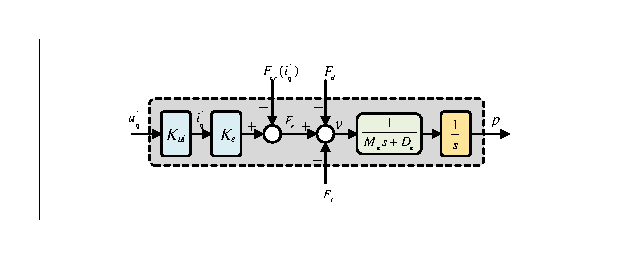
\includegraphics[width=12cm]{figures/电机数学模型}
	\caption{电机系统输入输出模型.}
	\label{电机系统模型}
\end{figure}

但是在实际工业环境中,精密直线运动平台的系统模型参数会随时间有一定的摄动,所以在实际应用中不得不考虑系统内部参数摄动情况。考虑模型参数摄动情况下,式(2.13)可进一步改写为
\begin{equation}
\label{2.14}
\begin{aligned}
\ddot{p}&=({{A}_{n}}+\Delta A)U+L \\ 
&={A}_{n}U+H  
\end{aligned}
\end{equation}
式中,

$A_n$指系统的名义参数;
$\Delta A$ 指的是系统参数的摄动,是未知部分,但假设其有界;
$H$指系统内部和外部的总扰动,表示为
\begin{equation}
\label{2.15}
H=\Delta AU+L
\end{equation}
假设总扰动$H$有界,即$H\le\mu$,$\mu$为一正常数。实际直线运动台中的扰动主要分为两种:一种是只依赖于系统状态,比如依赖于动子的位移和速度的摩擦力和定位力;一种是时变的扰动。为了更清晰地表示系统的扰动类型,式(\ref{2.15})可以进一步表示为:
\begin{equation}
H={{f}_{1}}(p,\dot{p},t)+{{f}_{2}}(p,\dot{p})
\end{equation}
式中,

$f_1(\cdot)$表示系统时变的扰动,包括纹波扰动、模型参数摄动、未知的外部扰动等时变的非线性扰动;

$f_2(\cdot)$表示系统时不变的扰动,包括定位力与摩擦力,分别依赖于PMLSMs动子的位移和速度。

对于定位力的建模,之前的文献中已经有所提及\cite{yao2011adaptive,song2017iterative},都将定位力建模成随位置变化的周期性函数,具体的数学表示为
\begin{equation}
F_{\text {cogging }}(p)=\sum_{i=1}^{\infty}\left(S_{i} \sin \left(\frac{2 i \pi p}{\tau}\right)+C_{i} \cos \left(\frac{2 i \pi p}{\tau}\right)\right)
\end{equation}
其中$\tau$为磁极距,$S_i$和$C_i$为常量系数。实际应用中,则往往选择公式中最重要的几个低阶项而忽略其他高阶项,例如$i$取从1到有界的值$n$。

从式(2.10)$\sim$(2.16)不难看出,PMLSMs控制系统要实现高精度的跟踪性能,最大的挑战就是要克服系统的总扰动$H$带来的影响。
%\subsection{定位力分析}

%\subsection{摩擦力分析}

\section{精密直线运动平台模型参数辨识}
参数辨识是指根据系统模型的结构对其相关参数进行辨识,往往是控制系统设计与实现的前提条件,对系统认识的越清楚越有利于控制器的设计。但是由于不同系统复杂程度的不同,系统辨识所需要的人力、物力也有很大区别。一般来说,根据参数估计是否实时进行,可将系统分为在线和离线辨识两种,这也是系统辨识中两个基本的概念。

1) 离线参数辨识要求把待辨识对象从系统中分离出来,然后给予辨识对象大量的输入,得到大量的输出信号,并保存输入输出信号。然后通过一定的算法对数据进行批处理,常用的有最小二乘、极大似然等,最后通过已知的模型结构进行系统参数辨识。

2) 在线参数辨识往往用于系统模型结构已知的情况,在设定初值之后,利用过去和现在的输入输出信息,采用递推的方式不断修正系统模型参数的估计值,这就要求辨识算法的运算速度足够快,能够保证在一个采样周期内计算出下一时刻的估计值,换句话说,如果辨识算法的运算需要的时间比较长,系统的采样频率必然只能维持在较低的水平,这对于高速高精度的系统来说是不能接受的。

在线辨识与离线辨识各有优缺点,总结如表\ref{在线辨识与离线辨识的优缺点比较}所示。
\begin{table}[H]
	\caption{在线辨识与离线辨识的优缺点比较.}
	\label{在线辨识与离线辨识的优缺点比较}
	\centering
	\setlength{\tabcolsep}{3mm}
	\begin{tabular}{ccc}
		\toprule[1.5pt]
		 &在线辨识  &离线辨识 \\
		\midrule
		%\hline
		优点&运算量小,可实时;&精度高,时间要求低\\
		缺点&精度低,时间要求高&占用存储空间,运算量大,耗时\\
		\bottomrule[1.5pt]
	\end{tabular}
\end{table}

本文被控对象为精密直线运动平台,常应用于高速、高精度工业环境中,因此,在线辨识方法不利于对系统特性的精确认识,这里采用离线辨识方法。

\subsection{离线辨识输入信号要求}
离线辨识要求输入信号满足持续激励条件和最优输入信号条件,其定义如下:
\begin{enumerate}
	\item[$\bullet$]持续激励条件,即在所观测周期内,系统的各阶模态能够对输入信号产生有效的响应,这要求输入信号的能量谱至少覆盖所关心的频带,同时能量大小足够激励各阶模态,这是保证辨识效果可信的先决条件\cite{刘金琨2013系统辨识理论及}。
	\item[$\bullet$]最优输入信号条件,更好的辨识精度,往往要求对输入信号类型、幅值、带宽等参数的选择尽可能达到最优,即最优输入信号设计问题。为了保证参数估计的有效性与最优输入信号条件联系起来,大多数最优输入准则都采用Fisher信息矩阵逆的标量函数作为评价函数J
	$$J=\phi(\textbf{\emph{$M_f$}}^{-1})$$
	其中,$\textbf{\emph{$M_f$}}$为Fisher信息矩阵,即$$\textbf{\emph{$M_f$}}=E_{\textbf{\emph{$y$}}|\textbf{\emph{$\theta$}}}\left\{\left[\frac{\partial \log p(\textbf{\emph{Y}}/\textbf{\emph{$\theta$}})}{\partial\textbf{\emph{$\theta$}}}\right]{\left[\frac{\partial \log p(\textbf{\emph{Y}}/\textbf{\emph{$\theta$}})}{\partial\textbf{\emph{$\theta$}}}\right]}^T\right\}$$
	式中$\textbf{\textit{Y}}$表示输入观测序列;$\textbf{\textit{$ \theta $}}$表示输入输出观测序列之间的参数向量。
	因此,当该评价函数达到最小时,可以认为输入信号最优。常见的满足最优输入信号条件的激励函数有白噪声、M序列和Chirp信号(频率随时间变化的正弦信号)。
\end{enumerate}
\subsection{基于频率响应函数的辨识方法}
基于频率响应函数(Frequency Response Function, FRF)的辨识方法是工程实际中最常用的辨识方法之一。输入激励信号在工程实际中常用的有两种:白噪声信号(或带有低通滤波器的白噪声信号)和Chirp信号。Chirp信号辨识实验往往需要的时间相对较长,精度较白噪声辨识会更高一些,但是在工程实际中,有时候为了快速得到模型信息,常采用白噪声信号辨识,由于本文所采用的控制方法的优势之一就是对模型信息要求不高,只需要知道系统大致的模型参数,即可实现高性能的控制,因此,在本文的辨识设计与实验中,均采用白噪声辨识的方法。关于辨识所采用的控制架构,一般有开环辨识、闭环辨识和半闭环辨识三种情况\cite{付雪微0有铁芯直线电机推力波动的分析与补偿方法研究}。

1)开环辨识。系统处于完全开环的状态下,直接给辨识对象输入激励信号,采集系统输出信号,然后根据系统自相关函数和互相关函数的傅里叶变换得出辨识对象的传递函数,即自功率谱和互功率谱,详见\cite{荣l1990系统辨识}。这里我们将根据考虑噪声情况的不同,分为两种情况介绍,如下图\ref{开环辨识控制框图}所示。

\begin{figure}[H]\centering
	\subfloat[含输出噪声]
	{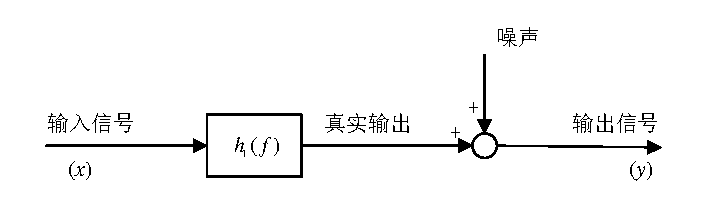
\includegraphics[width=12cm]{figures/开环测试输出噪声.pdf}
		\label{含输出噪声} }\\
	\subfloat[含输入噪声]
	{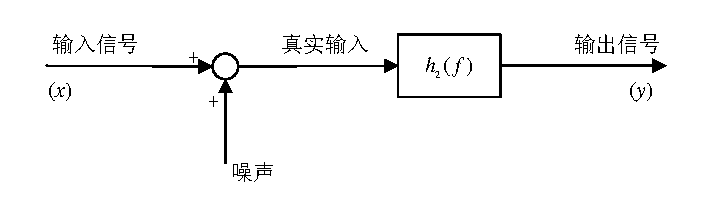
\includegraphics[width=12cm]{figures/开环测试输入噪声.pdf}
		\label{含输入噪声} }
	\caption{开环辨识控制框图}\label{开环辨识控制框图}
\end{figure}

如图\ref{含输出噪声}所示,当输出有噪声时,采用如下公式计算辨识对象的传递函数:
\begin{equation}
H_1=\frac{G_{XY}}{G_{XX}}
\end{equation}
式中,

$G_{XY}$为输入输出信号的互功率谱;
$G_{XX}$为输入信号的自功率谱。

如图\ref{含输入噪声}所示,当输入有噪声时,采用如下公式计算辨识对象的传递函数:
\begin{equation}
H_2=\frac{G_{YY}}{G_{YX}}
\end{equation}
式中,

$G_{YY}$表示输出信号的自功率谱;

$G_{YX}$表示输出输入信号的互功率谱。

2)闭环辨识。系统处于闭环(这里指位置闭环)状态下,假设系统没有噪声,闭环辨识的系统框图如图\ref{闭环辨识控制框图}所示,给系统输入经过低通滤波的白噪声,通过测得系统的输入输出信号,并经过离线批处理得到其闭环传递函数$G_2$,再根据提前人为设定的控制器C(最典型的为PID控制器)的参数,即可求得辨识对象P的传递函数,即$G_2=PC/(1+PC)$,则可得$P=G_2/(C-G_2C)$。需要注意的是,这里的白噪声的能量谱密度选取应该满足持续激励条件。
\begin{figure}[H]
	\centering
	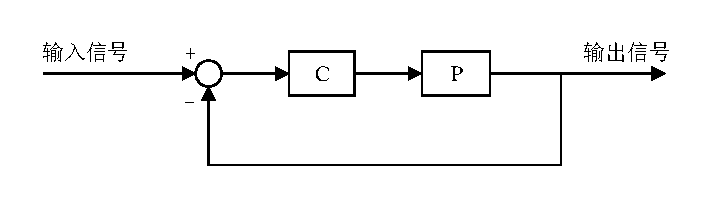
\includegraphics[width=12cm]{figures/闭环测试.pdf}
	\caption{闭环辨识控制框图.}
	\label{闭环辨识控制框图}
\end{figure}


3)半闭环辨识。半闭环辨识实际上也是一种闭环辨识方式,只不过输入信号的节点与闭环辨识相比产生了变化,如图\ref{半闭环辨识控制框图}所示。将位置参考信号设定为一个常数(这里是0),在位置环控制器输出后注入用于辨识的输入信号,然后通过位移传感器采集位置环输出信号,并经过离线批处理得到其传递函数$G_3$,即$G_3=P/(1+PC)$;进而结合提前设计好的控制器C的参数计算得出辨识对象P的传递函数,即$P=G_3/(1-G_3C)$;当$C$远大于1时,即$C\gg1$时,P退化为$P=1/C$,这是我们不期望的,因为此时的辨识精度会严重受影响,因此,我们在设计含闭环位置控制器的时候要尽量的设计较弱的闭环控制器,即其幅频响应在所关心的频率范围内要尽可能小。
\begin{figure}[H]
	\centering
	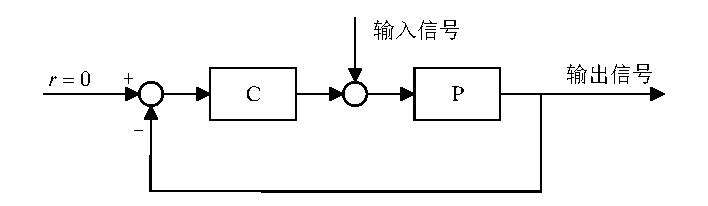
\includegraphics[width=12cm]{figures/半闭环测试.pdf}
	\caption{半闭环辨识控制框图.}
	\label{半闭环辨识控制框图}
\end{figure}
\subsection{基于频率响应函数的辨识结果}
本文综合考虑实际工程情况,采用半闭环辨识方法对精密直线运动实验平台进行了系统辨识,辨识所用的输入信号是由MATLAB/Simulink中自带的有限带宽的白噪声模块产生,相当于白噪声输出经过了低通滤波器,系统采样频率设为$5\,\text{kHz}$,在系统运行稳定之后,截取了$50\,\text{s}$时间的数据用于辨识所用的输入输出信号。数据处理基于前文所述方式,这里采用了MATLAB自带的tfestimate函数,最终得到的结果如图\ref{辨识结果}所示。
\begin{figure}[H]
	\centering
	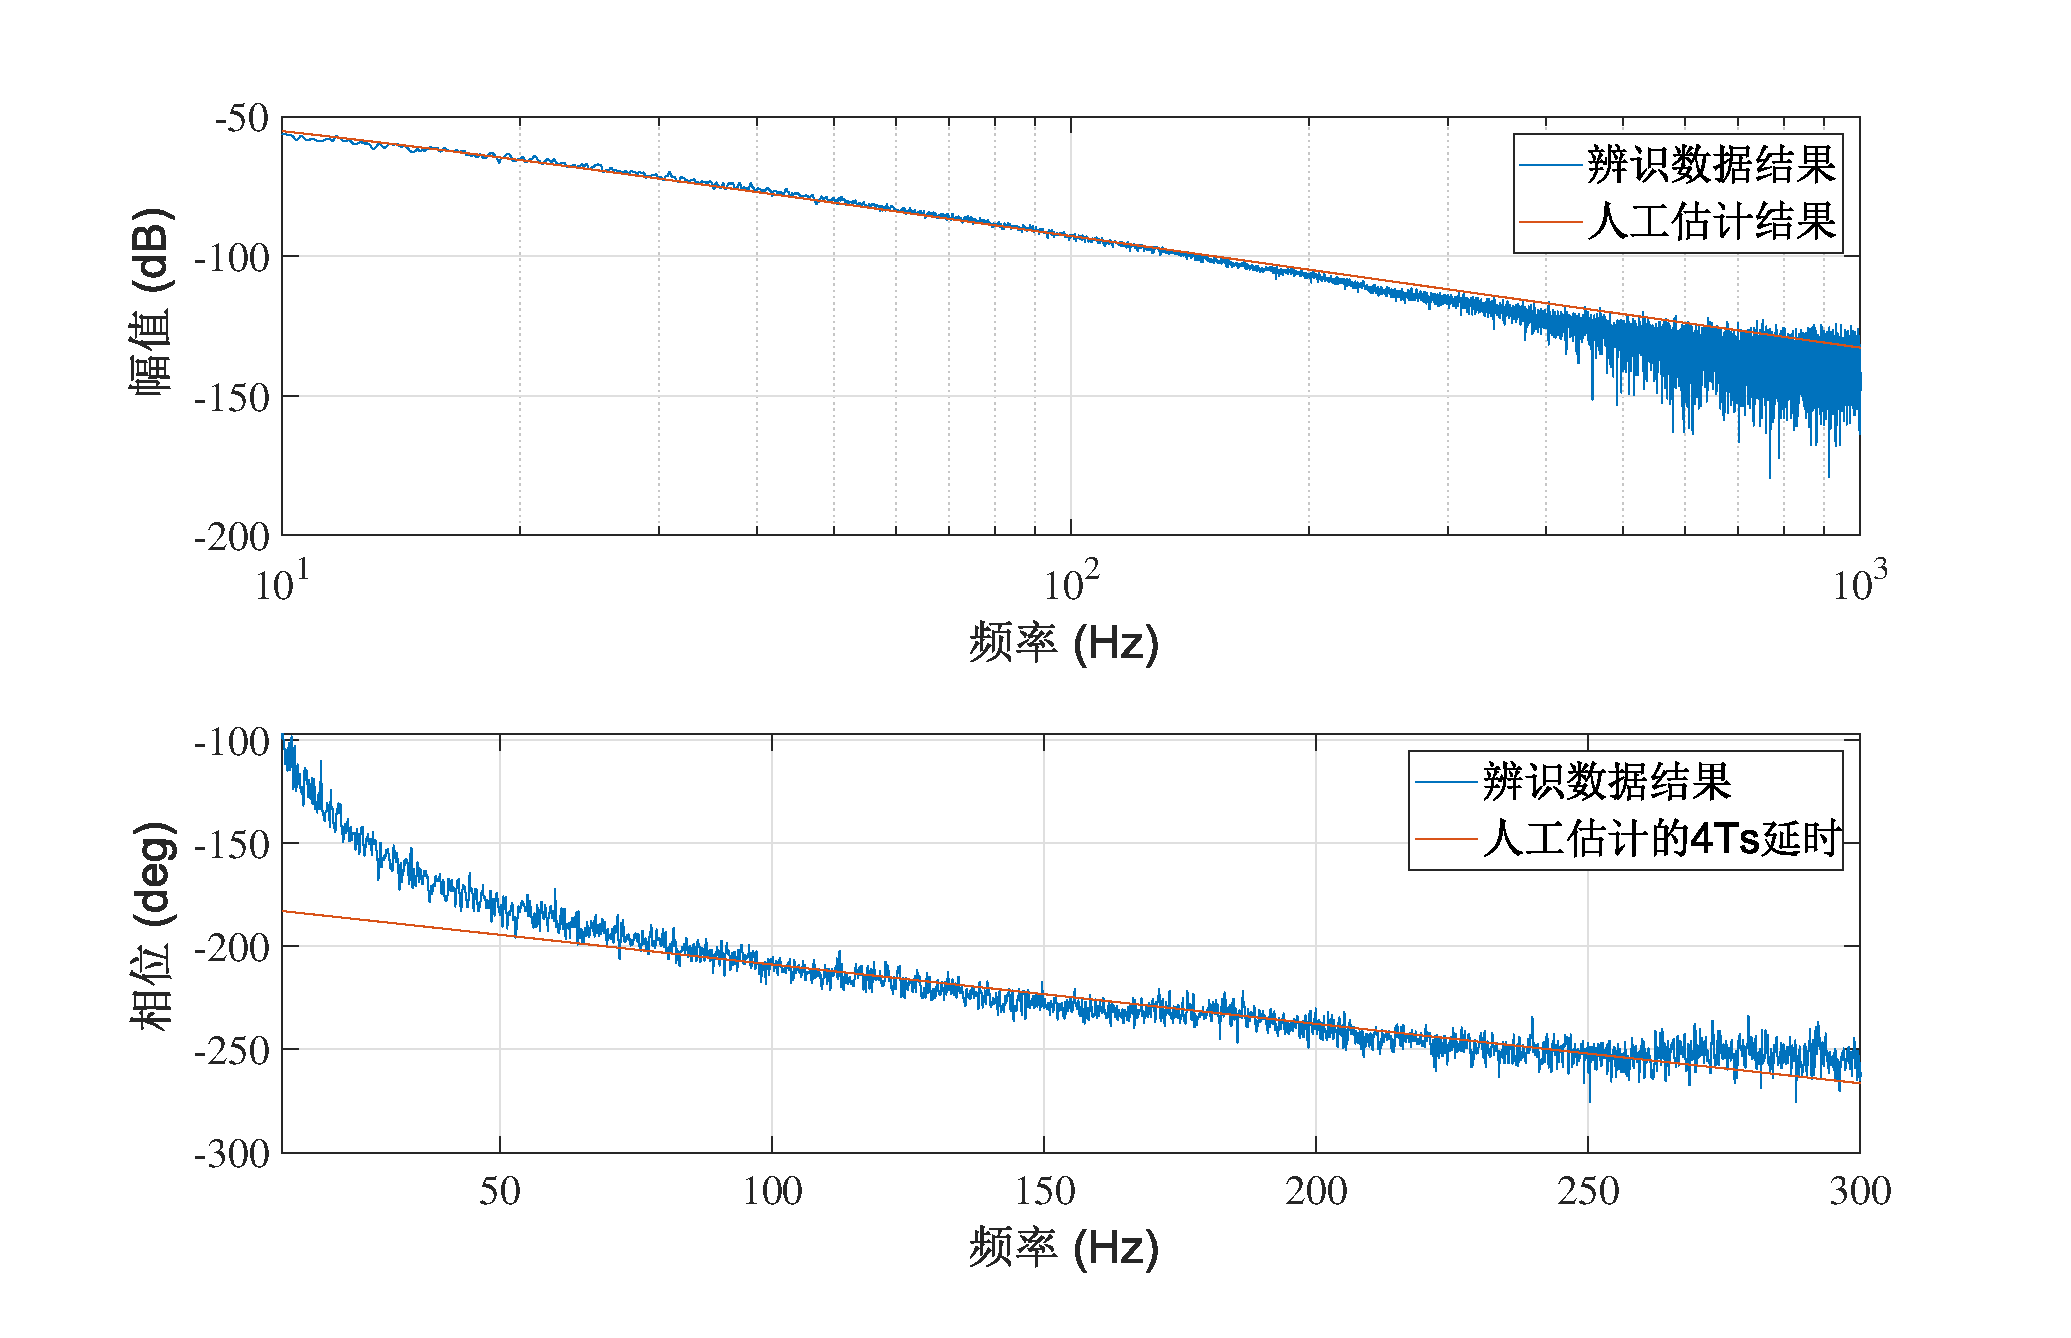
\includegraphics[width=12cm]{figures/辨识结果}
	\caption{辨识结果.}
	\label{辨识结果}
\end{figure}
图中,蓝色的线为实际辨识的数据,红色的线为辨识估计的数据。这里估计所采用的数学模型为最基础的二阶模型,如式(\ref{辨识公式})所示:
\begin{equation}
\label{辨识公式}
G(s)=\frac{1}{M_es^2+D_es}e^{-st_d}
\end{equation}
式中,由于辨识实际系统模型如图\ref{电机系统模型}所示,包含了驱动器部分,因此,辨识所得参数结果如下:

$M_e$为系统等效质量,这里为$\text{0.12$\,$Vs$^{2}$/m}$;

$D_e$为系统等效粘滞摩擦系数,这里为$\text{2.0$\,$Vs/m}$;

$t_d$为系统延时,这里为$\text{4$\,T_s$}$,即$\text{0.0008$\,$s}$。

从辨识结果来看,在300\,Hz以内,幅频曲线拟合的都比较好,超过300\,Hz,由于高频的未建模动态等因素,导致无法很好地拟合数据结果。相频曲线,从式(\ref{辨识公式})可知,估计采用的模型在$\text{s}$域内有两个极点,一个为0,另一个为$D_e/M_e$,即相位从-90°开始,在$\left|D_e/M_e\right|$\,Hz处下降90°,之后以斜率为$t_d$的直线变化,相对来说在300\,Hz以内,相频曲线较为理想。虽然高频无法很好地进行辨识,但辨识结果已经足以满足对于本文所涉及方法的要求,因为本文讨论的基于神经网络的一些方法对于模型的要求并不高,另外的一些补偿方法,也都会将模型的变化当做扰动的一种形式进行补偿。

此外,本文还对精密直线运动实验平台进行了定位力最大空间周期(即定位力的基频所对应的空间周期)的辨识,通过低速匀速运行,采集控制信号与位移信号,可以得到如图\ref{空间周期辨识}所示的结果,从图中很容易发现所标注的数据包含着定位力最大空间周期$\tau_{rip}=2\tau/3\,\text{mm}$的信息,其中$\tau$为实验平台PMLSM的极距($\tau=20\,\text{mm}$)。所标注出来的包含着几个非常常见的定位力的倍频所对应的空间周期,分别为$2\tau/3,\tau/3,\tau/4,\tau/6,2\tau/9$。
\begin{figure}[H]
	\centering
	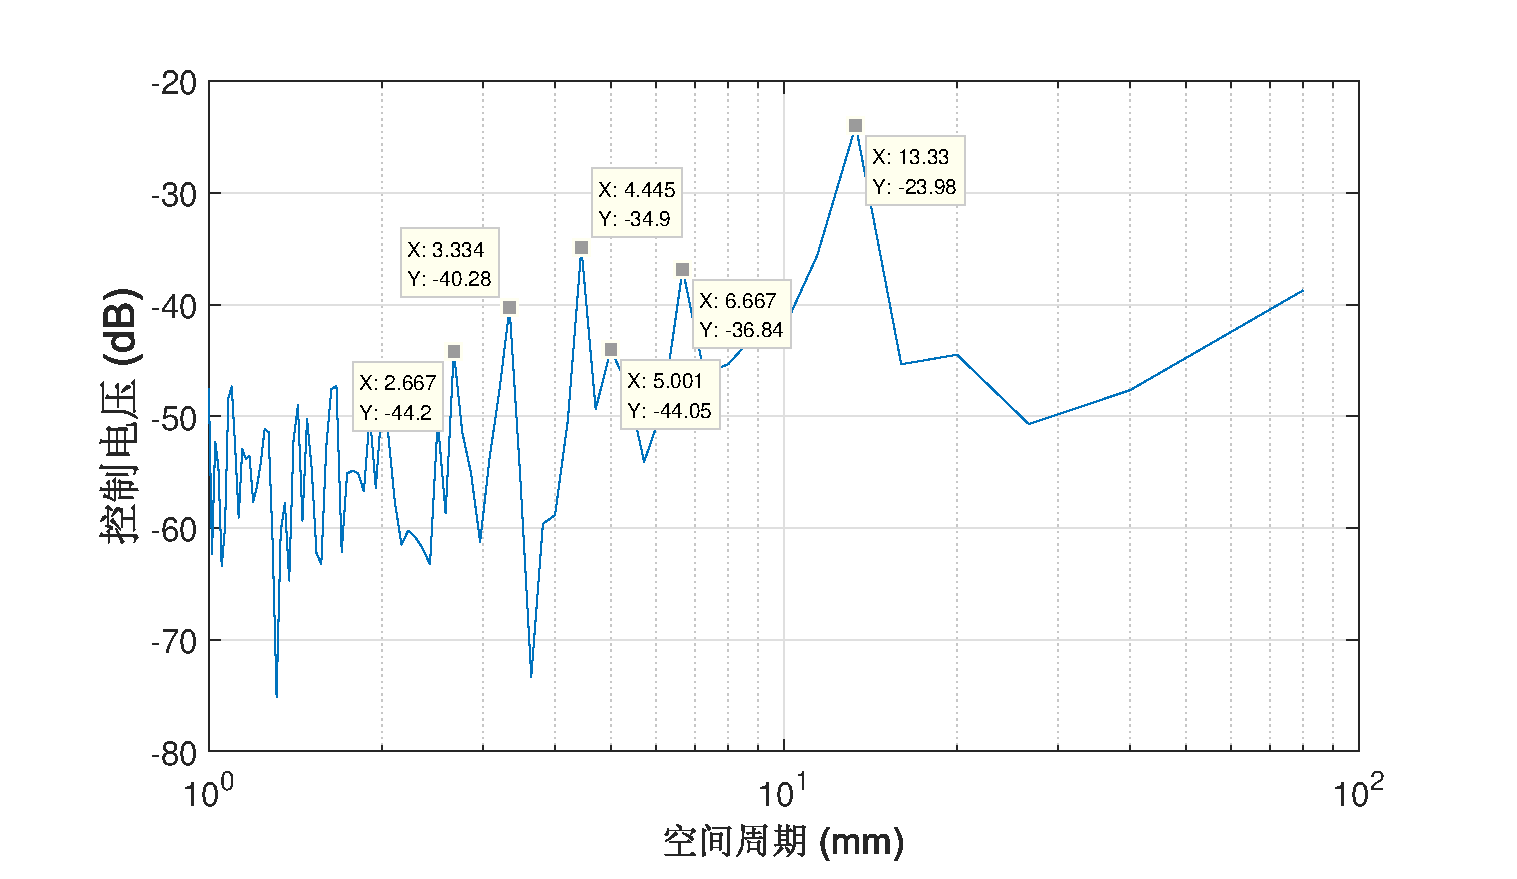
\includegraphics[width=12cm]{figures/空间周期辨识}
	\caption{定位力空间周期辨识.}
	\label{空间周期辨识}
\end{figure}
\section{本章小结}
本章首先介绍了精密直线运动平台系统工作原理,详细推导了PMLSMs的矢量变换控制原理。然后对精密直线运动平台动力学模型进行了详细介绍并提出了改进的扰动模型,其中,将系统扰动以集总扰动的形式进行了建模,为了方便后文控制方法的提出,进一步根据PMLSMs系统的特性,将集总扰动分为了时变的和时不变的两部分。此外,详细介绍了基于频率响应函数的系统辨识方法,详细介绍了离线开环辨识、闭环辨识和半闭环辨识三种辨识控制架构,并基于离线半闭环辨识控制架构对实验对象进行了辨识,得到了系统等效质量为$\text{0.12$\,$Vs$^{2}$/m}$,系统等效粘滞摩擦系数
为$\text{2.0\,Vs/m}$,系统延时为$\text{0.8$\,$ms}$,还对系统定位力的周期特性进行了辨识,得到其最大空间周期约为$13.33\,\text{mm}$,还可以发现,定位力的周期特性中,包含了2倍频、4倍频和6倍频的位置依赖扰动。这里系统模型特性为后续控制方法的研究提供了很好的基础。
